\chapter{중복도, 엔트로피, 제약 평형}

\lectureoverview{가능한 상태에 에너지가 부여되면 확률 분포는 열역학적 대상이 된다. 먼저 엔트로피 증가를 평형화와 연결하고 \(dE=T\,dS\)를 이용해 열이 흐르는 방향을 유도한다. 그런 다음 하나의 계를 동일한 계의 큰 복제 집합으로 바꾸고, 각 점유수 집합에 해당하는 배열의 수를 세어 그 중복도의 로그가 엔트로피에 \(N\)를 곱한 값임을 보인다. 따라서 평형은 제약 조건 아래에서 엔트로피를 최대화하는 문제다. 이를 풀려면 라그랑주 승수법이 필요하다.}

\section{세 가지 기본량}

계가 이용할 수 있는 이산 상태에 \(i\)라는 표지를 붙이자. 우선은 이산적인 경우를 다룬다. 위상공간 측도를 도입하지 않고도 상태의 수를 셀 수 있기 때문이다. 상태 \(i\)의 확률이 \(P_i\)이면 \begin{equation}
 \sum_i P_i=1.
 \label{eq:sm3-normalization}
\end{equation}그 상태의 에너지가 \(E_i\)일 때 평균 에너지는 \begin{equation}
 \overline E=\sum_iP_iE_i.
 \label{eq:sm3-mean-energy}
\end{equation}여기서 \emph{평균}이라는 말이 중요하다. 계가 어떤 미시 상태에서 \(\overline E\)의 에너지를 가져야 하는 것은 아니다. 이는 가능한 에너지 값들에 확률을 가중하여 구한 평균이다.

\begin{classroomqa}\classquestion{여기서 확률과 통계를 구분하는 유용한 차이가 있나요?}\lecturerresponse{확률은 가능한 결과를 설명하는 모형을 제공하고, 통계학은 보통 관측 자료에서 출발해 무엇을 추론할 수 있는지 묻는다. 여기서는 확률 분포를 사용하지만, 같은 평균은 통계 자료에서도 자연스럽게 나타난다. 수업 중 가벼운 문답에서 두 용어를 엄밀히 구별하지 않는 것은 그 차이가 뒤이어 나올 물리에 영향을 주지 않기 때문이다.
\lecturetimestamp{00:01:39--00:02:21}}\end{classroomqa}

분포의 엔트로피는
\begin{equation}
 S[P]=-\sum_iP_i\log P_i.
 \label{eq:sm3-entropy}
\end{equation}
이 표현은 음이 아니다. 확률이 양수이면 모두
\(0<P_i\leq1\)를 만족하므로 \(\log P_i\leq0\)이다. 통상적인 극한값 \(P_i\log P_i\to0\)은 \(P_i\to0\)일 때 적용된다.

\begin{figure}[t]\centering
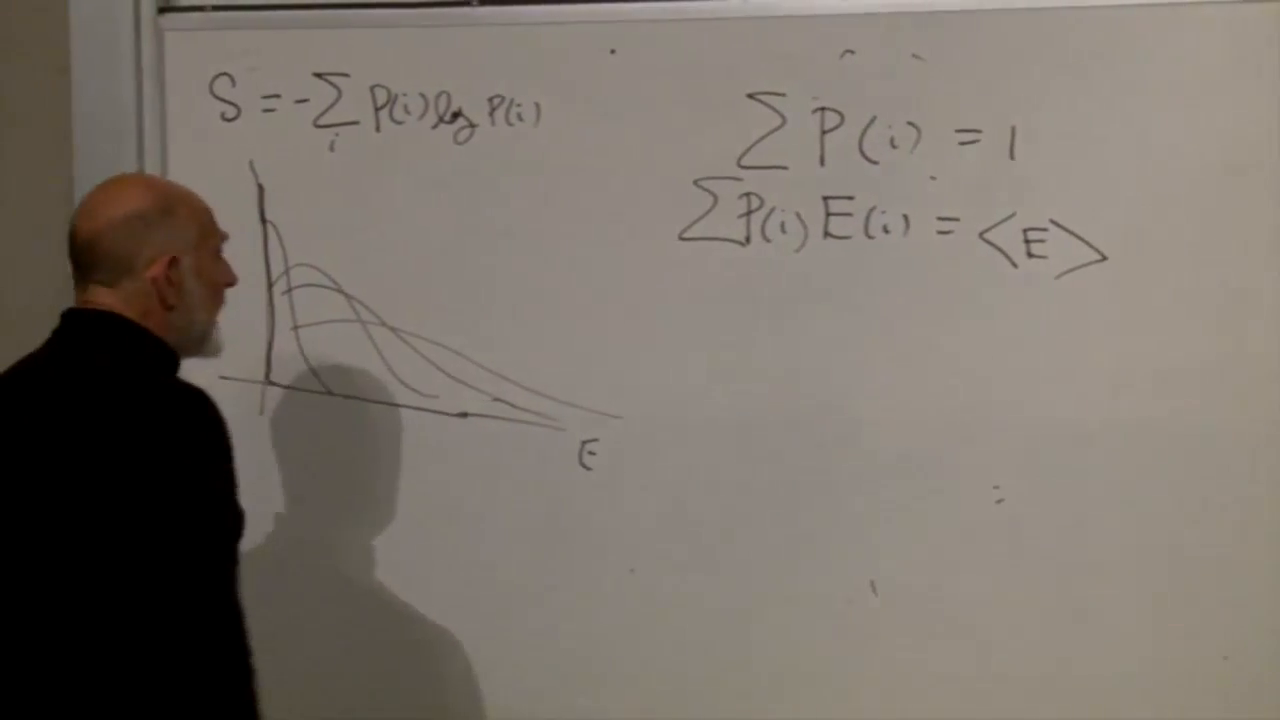
\includegraphics[width=0.88\textwidth]{lecture_03_figure_02.png}\caption{첫 번째 칠판에는 엔트로피, 정규화, 평균 에너지 공식과 평형 분포의 정성적인 모음이 함께 정리되어 있다.}\lectureframe{00:06:44}\end{figure}

\section{분포의 계로 나타낸 평형}

앞선 강의에서는 한 매개변수로 표시되는 평형 분포의 계를 살펴보았다. 이 계를 온도로 나타낼 수도 있지만, 지금은 평균 에너지 \(\overline E\)로 나타내는 편이 더 유용하다. 가능한 최저 에너지에서는 분포가 바닥 상태 하나에 집중된다.
\[
 P_i=\delta_{i0}.
\]이때 상태에 불확실성이 없으므로 \(S=0\)이다. 평형 분포가 더 많은 에너지 준위에 걸쳐 퍼질수록 평균 에너지와 엔트로피는 모두 증가한다.

이는 열적 계에 관한 진술이지, 임의로 만들 수 있는 모든 분포 계에 관한 진술은 아니다. 임의의 계라면 에너지가 커지는 동시에 분포가 좁아질 수도 있다. 여기서 유도할 평형 분포는 보통의 양의 온도 영역에서 그렇게 거동하지 않는다. 이 계를 따라서는
\begin{equation}
 \frac{dS}{d\overline E}>0.
 \label{eq:sm3-positive-temperature-branch}
\end{equation}스펙트럼에 상한이 있는 계에는 이 도함수가 음수가 되는 가지도 있을 수 있다. 그런 음의 온도 영역도 실제로 존재하지만, 여기서는 논의에서 제외한다.

열평형은 미시적인 정지 상태보다 더 넓은 뜻을 지닌다. 분자는 계속 움직이고, 충돌하며, 에너지를 주고받는다. 정지한 것은 거시적 기술이다. 분포에 순방향 변화가 더는 없고, 계의 서로 떨어진 부분 사이에 순 에너지 흐름도 더는 유지되지 않는다.

\section{열역학 법칙을 통계역학의 언어로}

제1법칙은 에너지 보존이다. 제2법칙에 따르면 고립된 거시계의 열역학적 엔트로피는 감소하지 않는다.
\begin{equation}
 \Delta S_{\mathrm{tot}}\geq0.
 \label{eq:sm3-second-law}
\end{equation}등호는 평형 상태나 이상적인 가역 변화를 나타내고, 자발적인 완화에서는 보통 엄격한 증가가 일어난다.

확률적 관점에서 완화가 일어나면 우리가 구별하는 거시적 대안들에 걸친 가중치가 퍼지는 경향이 있다. 여기에는 강의에서 강조한 단서가 필요하다. 우리는 \emph{거친 입자화}를 하고 있다. 정확한 해밀턴 시간발전은 세밀한 위상공간 엔트로피를 보존한다. 미시적 상관관계와 세부 사항을 더 이상 추적하지 않기 때문에 거시적 엔트로피가 증가한다. 이렇게 정보를 잃으면 축약된 기술은 더 넓어진다. 자발적으로 분포가 좁아진다면 측정도 하지 않은 채 미시적 정보를 알아낸 셈이 된다.

영 법칙은 계들이 열평형에 도달할 수 있고, 평형 관계가 추이적임을 말한다. \(A\)가 \(B\)와 평형을 이루고, \(B\)가 \(C\)와 평형을 이룬다면, \(A\)는 \(C\)와 평형을 이룬다. 온도는 이러한 추이성을 명확하게 보여 주는 수를 제공한다:
\[
 T_A=T_B,\qquad T_B=T_C
 \quad\Longrightarrow\quad
 T_A=T_C.
\]
평형 상태가 아니면 에너지는 온도가 더 높은 부분계에서 더 낮은 부분계로 흐른다. 온도가 같아지면 순흐름은 멈춘다. 이제 온도의 엔트로피 정의로부터 이 조작적 진술을 유도해 보자.

\section{에너지는 왜 뜨거운 곳에서 차가운 곳으로 흐르는가}

약하게 결합된 두 부분 계 \(A\)와 \(B\)를 생각하자. 각 부분 계는 내부적으로 평형 상태에 있지만 온도는 서로 다르다. 다음과 같이 기호를 정하자.
\begin{equation}
 T_B>T_A>0.
 \label{eq:sm3-temperature-order}
\end{equation}작은 에너지 교환이 일어나는 동안 전체 에너지 보존에 따라
\begin{equation}
 dE_A+dE_B=0.
 \label{eq:sm3-energy-conservation}
\end{equation}제2법칙에 따르면
\begin{equation}
 dS_A+dS_B\geq0.
 \label{eq:sm3-entropy-change}
\end{equation}내부적으로 평형인 각 부분 계에서 온도는 다음과 같이 정의된다.
\begin{equation}
 dE_X=T_X\,dS_X,
 \qquad X=A,B.
 \label{eq:sm3-temperature-differential}
\end{equation}\eqref{eq:sm3-energy-conservation}을 대입하면
\begin{equation}
 T_A\,dS_A+T_B\,dS_B=0,
\end{equation}따라서
\begin{equation}
 dS_B=-\frac{T_A}{T_B}\,dS_A.
 \label{eq:sm3-dsb}
\end{equation}이 결과를 \eqref{eq:sm3-entropy-change}에 넣으면
\begin{align}
 dS_{\mathrm{tot}}
 &=dS_A-\frac{T_A}{T_B}dS_A\\
 &=\frac{T_B-T_A}{T_B}\,dS_A\geq0.
 \label{eq:sm3-flow-entropy}
\end{align}\(T_B-T_A>0\)이고 \(T_B>0\)이므로 자발적인 교환에는 다음 조건이 필요하다.
\[
 dS_A>0.
\]\eqref{eq:sm3-temperature-differential}에 따라
\begin{equation}
 dE_A=T_A\,dS_A>0,
 \qquad
 dE_B=-dE_A<0.
 \label{eq:sm3-hot-to-cold}
\end{equation}에너지는 더 뜨거운 부분 계인 \(B\)에서 더 차가운 부분 계인 \(A\)로 흘렀다. 여기서 열은 단순히 이동 중인 에너지다. \(T_A=T_B\)가 될 때까지 흐름은 계속된다. 그때는 1차 엔트로피 변화가 어느 한쪽 방향도 더는 선호하지 않는다.

같은 결과를 한 줄로 쓸 수 있다.
\begin{equation}
 dS_{\mathrm{tot}}
 =dE_A\left(\frac{1}{T_A}-\frac{1}{T_B}\right)\geq0.
 \label{eq:sm3-compact-flow}
\end{equation}역온도 차의 부호가 \(dE_A\)의 부호를 결정한다. 이 간결한 형태는 뒤에서 정준 앙상블과 자연스럽게 연결된다.

\begin{classroomqa}\audiencequestion{이 논증은 \(A\)와 \(B\)가 각각 이미 내부 평형 상태라고 가정하나요?}\lecturerresponse{그렇습니다. 하나의 \(T_A\) 또는 \(T_B\)를 부여하는 것 자체가 그 가정을 뜻합니다. 부분 계가 내부 평형이 아니라면, 더 작은 영역들로 나누어 온도를 정의할 수 있는 곳마다 국소적으로 이 논증을 적용하면 됩니다. 그러면 전체적인 완화는 그 영역들 사이의 에너지 교환을 모아 설명할 수 있습니다.
\lecturetimestamp{00:24:38--00:25:22}}\end{classroomqa}

\section{상태란 무엇인가?}

평형 확률을 묻기 전에 표지 \(i\)가 무엇을 뜻하는지 알아야 한다. 미시 상태란 물리 법칙이 허용하는 범위에서 계를 가장 완전하게 규정한 것이다. 고전역학에서는 모든 입자의 위치와 운동량을 떠올리면 된다. 양자역학에서 상태는 그 대신 완전한 양자 상태를 뜻한다. 불확정성 원리 때문에 고전적인 위치와 운동량을 모두 동시에 정확히 지정할 수는 없다.

유한한 상자 안의 양자계에서는 관련 상태 수가 이산적일 수 있다. 적절한 극한에서 촘촘히 놓인 양자 상태의 합이 위상공간 적분으로 바뀌면 고전 통계역학이 얻어진다. 이 극한 과정에서는 연속적인 엔트로피를 무차원으로 만들 위상공간 셀도 도입된다. 단순히 합 기호를 적분 기호로 바꾸는 것만으로 얻어지는 것은 아니다.

\begin{classroomqa}\audiencequestion{기체에서는 모든 분자의 위치와 운동량을 상태로 생각해야 하나요?}\lecturerresponse{고전적인 관점에서는 그렇다. 더 일반적으로 상태란 물리 법칙이 허용하는 범위에서 원칙적으로 계에 대해 알 수 있는 모든 것을 뜻한다. 양자역학에서는 이러한 최대한의 기술 방식이 달라지고, 유한 부피에서의 상태 수는 이산적으로 세어진다. 양자 합에서 고전 적분을 얻는 것은 실제 극한 논증이지, 한 줄짜리 치환이 아니다.
\lecturetimestamp{00:25:31--00:27:38}}\end{classroomqa}

\section{복제 계로 이루어진 열저장고}

이제 핵심 질문을 피할 수 없다. 평형이 성립한 뒤 \(P_i\)를 결정하는 것은 무엇인가?

부분 계를 매우 큰 열저장고와 접촉시켜 보자. 에너지는 오갈 수 있지만, 열저장고에는 자유도가 아주 많으므로 소량의 에너지 이동은 온도를 거의 바꾸지 않는다. 특히 편리한 열저장고는 부분 계 자체를 약하게 결합한 복제 계들로 많이 모아 구성할 수 있다. 복제 계 하나가 연구 대상인 계이고, 나머지는 그 환경을 이룬다.

이 구성은 실제 거시계를 본뜨는 경우가 많다. 거의 균일한 큰 물체를 비슷한 여러 셀로 나눈다고 하자. 각 셀은 부분 계이고 나머지 셀들은 그 셀의 열저장고 역할을 한다. 복제 계의 전체 수를 \(N\)로 나타내자. 수업 중 시연에서는 복제 계 아홉 개와 색으로 구분한 상태 표지 세 개를 사용하지만, 계수 결과는 그 구체적인 수와 무관하다.

상태 \(i\)에 있는 복제 계의 수를 \(n_i\)로 두자. 이를 \emph{점유수}라 한다. 가능한 에너지 준위가 무한히 많더라도 전체 에너지가 유한하면 매우 높은 준위의 점유수는 대부분 무시할 수 있거나 0이다.

첫 번째 제약은 복제 계의 수다.
\begin{equation}
 \sum_i n_i=N.
 \label{eq:sm3-number-constraint}
\end{equation}두 번째 제약은 총에너지다.
\begin{equation}
 \sum_i n_iE_i=N\overline E.
 \label{eq:sm3-total-energy-constraint}
\end{equation}우변은 가산적이다. 통계적 상태를 그대로 유지하면서 복제 계의 수를 두 배로 늘리면 총에너지는 두 배가 되지만 복제 계 하나당 평균 에너지는 \(\overline E\)로 유지된다.

\begin{classroomqa}\audiencequestion{복제 계 구성에서도 에너지 제약을 만족해야 하나요?}\lecturerresponse{그렇다. 점유수의 합은 \(N\)이어야 하고, 점유수에 에너지를 가중해 합한 값은 고정된 총에너지 \(N\overline E\)와 같아야 한다. 뒤에서 엔트로피 최대값을 제한하는 조건은 바로 이 두 가지다.
\lecturetimestamp{00:37:12--00:39:54}}\end{classroomqa}

무작위로 선택한 복제 계가 상태 \(i\)를 차지할 확률은 그 상대 도수다.
\begin{equation}
 P_i=\frac{n_i}{N},
 \qquad
 n_i=NP_i.
 \label{eq:sm3-frequency-probability}
\end{equation}

\begin{figure}[t]\centering
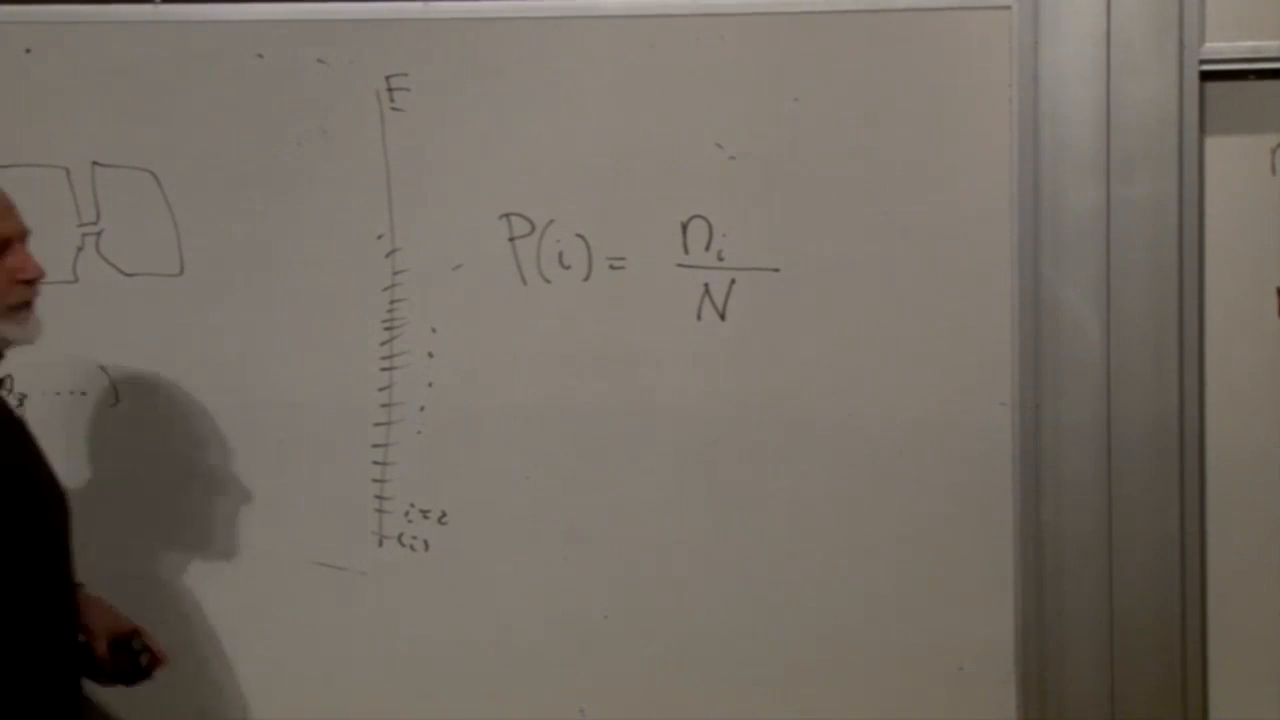
\includegraphics[width=0.82\textwidth]{lecture_03_figure_03.png}\caption{에너지 준위 그림과 점유 비율을 확률로 보는 해석 \(P_i=n_i/N\).}\lectureframe{00:41:40}\end{figure}

\begin{classroomqa}\audiencequestion{칠판의 표기 \(N(i)\)는 \(n_i\)와 다른 뜻인가요?}\lecturerresponse{아니다. 둘 다 상태 \(i\)의 점유수를 나타낸다. 일관되게 \(n_i\)를 사용하고 복제 계의 총수에는 대문자 \(N\)를 쓰기로 하자.
\lecturetimestamp{00:41:28--00:41:33}}\end{classroomqa}

\eqref{eq:sm3-number-constraint}와 \eqref{eq:sm3-total-energy-constraint}를 \(N\)로 나누면 확률 제약 조건이 다시 나온다.
\begin{equation}
 \sum_iP_i=1,
 \qquad
 \sum_iP_iE_i=\overline E.
 \label{eq:sm3-probability-constraints}
\end{equation}따라서 앙상블의 상대 도수 해석으로 처음에 세웠던 방정식을 다시 얻었다.

\section{점유 패턴의 중복도}

점유수 집합 \(\{n_i\}\)를 고정하자. 서로 구별되는 \(N\)개의 복제 계를 상태들에 배정해 정확히 그 집합을 실현하는 방법은 몇 가지일까? 답은 다항계수다.
\begin{equation}
 C(\{n_i\})=\frac{N!}{\prod_i n_i!}.
 \label{eq:sm3-multiplicity}
\end{equation}분모가 생기는 이유를 살펴보자. 먼저 표지가 붙은 복제 계 \(N\)개를 모두 \(N!\)가지 순서로 배열한다. 같은 상태에 있는 \(n_i\)개의 복제 계끼리 자리를 바꾸어도 새로운 점유 배정이 되지 않으므로 각 상태마다 \(n_i!\)로 나눈다.

\begin{figure}[t]\centering
\includegraphics[width=0.88\textwidth]{lecture_03_figure_04.png}\caption{칠판에 적힌 다항 중복도 \(C=N!/\prod_i n_i!\).}\lectureframe{00:46:55}\end{figure}

점유되지 않은 준위는 \(0!=1\)이므로 문제가 되지 않는다. 모든 복제 계가 한 상태에 있다면
\[
 C=\frac{N!}{N!}=1,
\]예상한 대로다. 세 복제 계가 서로 다른 세 지정 상태를 차지한다면
\[
 C=\frac{3!}{1!\,1!\,1!}=6.
\]두 복제 계가 서로 다른 지정 상태 두 개를 차지하는 경우에는 두 가지 배정이 나온다. 표지가 붙은 두 복제 계가 각각 어느 상태를 차지하는지를 맞바꾸면 된다.

\begin{classroomqa}\audiencequestion{두 제약 조건을 만족하는 점유수 집합이 여러 개일 수 있나요?}\lecturerresponse{대개 여러 집합이 가능하다. 식 \eqref{eq:sm3-multiplicity}은 먼저 제약 조건을 만족하는지 따지지 않고, 고정된 한 집합 \(\{n_i\}\)에 대한 배열 수를 센다. 다음 단계에서는 제약 조건과 양립하는 모든 집합을 비교해 중복도가 가장 큰 것을 찾는다.
\lecturetimestamp{00:48:07--00:48:43}}\end{classroomqa}

통계적 가정은 고립된 설정과 양립하는 미시적 배정들을 동등하게 취급한다는 것이다. 따라서 더 많은 배정으로 실현되는 거시적 점유 패턴이 더 높은 확률을 갖는다. \(N\)가 클 때 비율 \(n_i/N\)의 분포는 뚜렷한 최빈값 주위에 집중된다. 평형 비율은 \eqref{eq:sm3-number-constraint}와 \eqref{eq:sm3-total-energy-constraint}를 만족하는 조건 아래 \(C\)을 최대화하는 값이다.

\section{스털링 근사}

계승은 \(N\)이 거시적인 값에 도달하기 훨씬 전부터 엄청나게 커지므로, 로그를 취해 다룬다. 다음 식에서 시작하자.
\begin{equation}
 \log N!=\sum_{x=1}^{N}\log x.
 \label{eq:sm3-log-factorial-sum}
\end{equation}
\(N\)이 클 때 이 합은 \(\log x\) 곡선 아래의 넓이로 근사된다.
\begin{align}
 \log N!
 &\simeq\int_1^N\log x\,dx\\
 &=\left[x\log x-x\right]_1^N\\
 &=N\log N-N+1.
 \label{eq:sm3-stirling-integral}
\end{align}
부정적분은 다음 식에서 바로 구할 수 있다.
\[
 \frac{d}{dx}(x\log x-x)=\log x.
\]
계의 크기에 비례하는 선도 차수에서는 가산 상수를 생략해도 된다.
\begin{equation}
 \log N!\simeq N\log N-N.
 \label{eq:sm3-stirling-log}
\end{equation}
양변을 지수화하면 강의에서 사용한 간단한 형태를 얻는다.
\begin{equation}
 N!\simeq N^N e^{-N}.
 \label{eq:sm3-stirling-simple}
\end{equation}

\begin{figure}[t]\centering
\includegraphics[width=0.88\textwidth]{lecture_03_figure_05.png}\caption{합 \(\log x\)을 적분으로 바꾸어 유도한 스털링 근사의 선도항.}\lectureframe{01:03:45}\end{figure}

\begin{classroomqa}\audiencequestion{하한에서 \(x\log x-x\)을 계산하면 \(+1\)가 더 남지 않나요?}\lecturerresponse{그렇다. 식 \eqref{eq:sm3-stirling-integral}에는 그 상수가 들어 있다. \(N\to\infty\)일 때 \(N\)에 비례하는 항들에 비하면 무시할 수 있으므로 선도 근사식에서는 생략한다. 합은 반드시 \(x=1\)에서 시작해야 한다. \(\log0\)는 정의되지 않는다.
\lecturetimestamp{01:04:12--01:04:35}}\end{classroomqa}

\begin{classroomqa}\audiencequestion{\(\sqrt{N}\)에 비례하는 인자도 빠진 것 아닌가요?}\lecturerresponse{그렇다. 더 정확한 점근식은 다음과 같다.
\[
 N!\sim\sqrt{2\pi N}\left(\frac{N}{e}\right)^N.
\]로그를 취하면 \(\tfrac12\log(2\pi N)\)만 추가되는데, 이는 \(N\log N-N\)에 비해 비가산적이다. 유한한 \(N\)에서 확률을 정확히 계산할 때는 중요하지만, 거시계의 엔트로피를 선도 차수에서 계산할 때는 중요하지 않다.
\lecturetimestamp{01:04:35--01:05:40}}\end{classroomqa}

\eqref{eq:sm3-multiplicity}의 분모에 스털링 근사를 적용할 때도 주의해야 한다. 열역학적 극한에서 극한 확률이 양수인 상태들은 \(n_i=NP_i\)를 만족하므로, 그 점유수는 \(N\)에 비례해 커진다. 점유수가 매우 작거나 사라지는 상태는 유한한 에너지 절단을 도입해 다룬 뒤 극한을 취해 복원할 수 있다. 생략한 차수 낮은 항들은 선도적인 광범위 엔트로피에 영향을 주지 않는다.

\section{중복도의 로그가 엔트로피다}

분자와 거시적으로 점유된 모든 분모 인자에 \eqref{eq:sm3-stirling-simple}를 적용하면
\begin{equation}
 C\simeq
 \frac{N^Ne^{-N}}
 {\prod_i n_i^{\,n_i}e^{-n_i}}.
 \label{eq:sm3-c-stirling}
\end{equation}\(\sum_i n_i=N\)이므로 선도 지수 인자들이 상쇄된다.
\begin{equation}
 C\simeq\frac{N^N}{\prod_i n_i^{\,n_i}}.
 \label{eq:sm3-c-leading}
\end{equation}곱보다 로그를 최대화하기가 쉽고 로그는 단조 함수이므로 두 경우의 최댓값은 같은 점유 패턴에서 얻어진다.
\begin{equation}
 \log C=N\log N-\sum_i n_i\log n_i.
 \label{eq:sm3-logc-occupations}
\end{equation}이제 \(n_i=NP_i\)를 대입하면
\begin{align}
 \log C
 &=N\log N-\sum_iNP_i\log(NP_i)\\
 &=N\log N-N\sum_iP_i\log N
   -N\sum_iP_i\log P_i\\
 &=-N\sum_iP_i\log P_i,
 \label{eq:sm3-logc-entropy-derivation}
\end{align}정규화 조건에 의해 두 \(N\log N\) 항이 상쇄된다. 따라서 \(N\)의 선도 차수에서
\begin{equation}
 \boxed{\log C=NS}.
 \label{eq:sm3-logc-ns}
\end{equation}

\begin{figure}[t]\centering
\includegraphics[width=0.88\textwidth]{lecture_03_figure_06.png}\caption{칠판 계산: \(\log C=N\log N-\sum_i n_i\log n_i\)를 \(-N\sum_iP_i\log P_i=NS\)와 연결한다.}\lectureframe{01:16:10}\end{figure}

이 관계는 이 장의 핵심이다. 엔트로피는 계수 문제에 별도로 덧붙인 무관한 양이 아니다. 엔트로피는 복제 계 하나당 중복도를 로그로 측정한 것이다. 따라서 선도 차수에서 미시적 배열의 수를 최대화하는 것은 복제 계 하나의 엔트로피를 최대화하는 것과 같다.

\begin{classroomqa}\audiencequestion{점유수가 모두 같을 때 중복도가 가장 크지 않나요?}\lecturerresponse{어떤 상태도 특별히 구별되지 않고 유한한 상태 집합에서 \(\sum_i n_i=N\)만 부과될 때는 균일 분포가 된다. 고정 에너지 제약이 답을 바꾸는 이유는 \(E_i\)의 값이 서로 다르기 때문이다. 일반적으로 점유수를 같게 하면 지정된 평균 에너지를 얻을 수 없다.
\lecturetimestamp{01:17:07--01:18:20}}\end{classroomqa}

\begin{classroomqa}\audiencequestion{수 \(N\)는 크지만, 분모의 모든 \(n_i\)에 스털링 근사를 적용해도 되는 이유는 무엇인가?}\lecturerresponse{극한 확률이 양수인 각 상태에서는 \(n_i=NP_i\)가 \(N\)에 비례해 커집니다. 먼저 유한한 에너지 범위만 남겨 그 범위에서 \(N\)가 커지는 극한을 취한 다음, 에너지 범위를 넓힐 수 있습니다. 꼬리 부분의 희소한 상태들은 별도의 유한한 보정이 필요하지만, 선도적인 광범위 엔트로피를 바꾸지는 않습니다.
\lecturetimestamp{01:18:23--01:19:28}}
\end{classroomqa}

\begin{classroomqa}\audiencequestion{앞서 말한 거친 입자화가 바로 이 큰 \(N\) 근사를 뜻하나요?}\lecturerresponse{아니다. 열역학적 극한은 큰 점유수와 점근적 계수를 다룬다. 거친 입자화는 미시적 분해능을 잃거나 의도적으로 버리는 일이다. 거시적 통계역학에서 둘 다 자주 쓰이지만, 서로 다른 연산이다.
\lecturetimestamp{01:19:29--01:19:46}}\end{classroomqa}

\begin{classroomqa}\audiencequestion{\(\log C=N\log N-\sum_i n_i\log n_i\)이므로 두 번째 항을 최대화하는 대신 최소화해야 하나요?}\lecturerresponse{그렇다. \(N\)를 고정하면 \(\log C\)를 최대화하는 것은 \(\sum_i n_i\log n_i\)를 최소화하는 것과 같다. \(n_i=NP_i\)를 대입하면 고정된 \(N\log N\) 항들이 상쇄되고 \(-N\sum_iP_i\log P_i=NS\)만 남는다. 따라서 이를 양의 엔트로피 \(S\)를 최대화하는 것으로 표현하는 편이 더 자연스럽다.
\lecturetimestamp{01:19:48--01:20:55}}\end{classroomqa}

\begin{classroomqa}\audiencequestion{대칭성을 이용해 곧바로 모든 \(n_i\)를 같게 두면 안 되나요?}\lecturerresponse{그렇게 하면 에너지 표지를 무시하게 된다. 정규화 제약은 상태들을 대칭적으로 다루지만 \(\sum_iP_iE_i=\overline E\)는 그렇지 않다. 에너지가 다른 상태들은 서로 다르게 기여한다. 에너지 제약이 바로 비균일한 평형 분포를 결정한다.
\lecturetimestamp{01:21:15--01:21:41}}\end{classroomqa}

\section{최대 엔트로피 문제}

이제 통계역학의 규칙을 모호함 없이 쓸 수 있다. 확률 \(P_i\)를 변화시켜
\begin{equation}
 S[P]=-\sum_iP_i\log P_i
 \label{eq:sm3-maximize-entropy}
\end{equation}를 최대화한다. 단, 다음 조건을 만족해야 한다.
\begin{equation}
 \sum_iP_i=1,
 \qquad
 \sum_iP_iE_i=\overline E.
 \label{eq:sm3-maxent-constraints}
\end{equation}최대화된 확률은 큰 복제 앙상블에서 뚜렷하게 선호되는 점유 비율을 준다. 점유수는 요동하지만 \(N\)가 커질수록 상대 편차는 줄어들어 비율 \(n_i/N\)가 잘 정의된 열역학적 확률이 된다.

\begin{classroomqa}\audiencequestion{\(E_i\)는 고정된 상태 에너지이고, 제약 조건에는 별도로 주어진 총에너지를 쓰나요?}\lecturerresponse{그렇다. 스펙트럼 \(\{E_i\}\)는 부분 계의 고유한 성질이다. 복제 계 전체의 총에너지는 고정되어 있지만, 에너지는 복제 계들 사이에서 계속 이동한다. 총에너지를 \(N\)로 나누면 복제 계 하나의 평균 에너지 \(\overline E\)가 정해질 뿐, 개별 미시적 실현에서 복제 계의 에너지가 정해지는 것은 아니다.
\lecturetimestamp{01:26:12--01:27:07}}\end{classroomqa}

문제는 쉽게 쓸 수 있지만 아직 풀리지는 않았다. 제약 조건이 두 개인 극값 문제이므로 수학적 도구가 하나 더 필요하다.

\section{라그랑주 승수}

제약이 없는 함수 \(F(x_1,x_2,\ldots)\)의 정지점은 다음을 만족한다.
\begin{equation}
 \frac{\partial F}{\partial x_i}=0
 \qquad\text{for every }i.
 \label{eq:sm3-unconstrained-stationary}
\end{equation}이제 추가로 다음 조건을 요구하자.
\begin{equation}
 G(x_1,x_2,\ldots)=0.
 \label{eq:sm3-one-constraint}
\end{equation}

\begin{classroomqa}\audiencequestion{그림의 좌표가 \(x\)와 \(y\)라면 \(x\)는 무엇을 뜻하나요?}\lecturerresponse{여기서 \(x\)은 좌표 벡터 전체 \((x_1,x_2,\ldots)\)를 간단히 나타낸 것이다. 이차원 그림에서는 성분이 \(x\)와 \(y\)뿐이다. 나중에는 성분이 확률 \(P_1,P_2,\ldots\)가 된다.
\lecturetimestamp{01:30:12--01:30:20}}\end{classroomqa}

기하학적으로 보면 곡면 \(F=\text{constant}\)은 등고선도이고, \(G=0\)은 계가 따라 움직일 수 있는 곡선이다. 제약된 극값은 \(F\)의 한 등고선이 제약 곡선에 접할 때 생긴다. 그 지점에서 기울기 벡터들은 서로 평행하다.
\begin{equation}
 \nabla F=-\lambda\nabla G
 \label{eq:sm3-parallel-gradients}
\end{equation}어떤 수 \(\lambda\)에 대하여 성립한다.

\begin{figure}[t]\centering
\includegraphics[width=0.88\textwidth]{lecture_03_figure_07.png}\caption{칠판에 그린 등고선의 기하학적 관계와 확장 함수 \(F'=F+\lambda G\). 접점에서 제약된 극값이 생긴다.}\lectureframe{01:37:10}\end{figure}

확장 함수
\begin{equation}
 F'=F+\lambda G
 \label{eq:sm3-augmented-function}
\end{equation}를 정의하고 보통의 정지 조건을 요구하면 식 \eqref{eq:sm3-parallel-gradients}를 얻을 수 있다.
\begin{equation}
 \frac{\partial F'}{\partial x_i}=0.
 \label{eq:sm3-augmented-stationarity}
\end{equation}승수 \(\lambda\)는 처음에는 미지수다. 그렇다고 연립 문제가 미정인 것은 아니다. 원래의 제약 조건 \(G=0\)이 방정식 하나를 더 제공한다.

\begin{classroomqa}\classquestion{\(G\)에 비례하는 항을 더하면 왜 제약된 점에서 정지하게 되나요?}\lecturerresponse{제약된 극값에서는 \(G=0\)에 접하는 방향으로 움직여도 \(F\)가 1차에서 변하지 않는다. 남은 기울기는 제약에 수직인 방향뿐이다. \(\nabla G\)는 바로 그 수직 방향을 가리키므로 적절한 \(\lambda\)를 택해 그 기울기를 상쇄할 수 있다.
\(\nabla F+\lambda\nabla G=0\).
\lecturetimestamp{01:35:06--01:35:32}}\end{classroomqa}

\section{두 변수 예제}

다음을 최소화하자.
\begin{equation}
 F(x,y)=\frac{x^2+y^2}{2}
 \label{eq:sm3-example-f}
\end{equation}단, 다음 조건을 만족해야 한다.
\begin{equation}
 x+y=1.
 \label{eq:sm3-example-constraint}
\end{equation}제약 조건을 \(G=x+y-1=0\)으로 쓰고 다음을 구성한다.
\begin{equation}
 F'=\frac{x^2+y^2}{2}+\lambda(x+y-1).
 \label{eq:sm3-example-augmented}
\end{equation}정지 조건은 다음과 같다.
\begin{align}
 \frac{\partial F'}{\partial x}&=x+\lambda=0,\\
 \frac{\partial F'}{\partial y}&=y+\lambda=0.
 \label{eq:sm3-example-derivatives}
\end{align}따라서 \(x=y=-\lambda\)이다. 남은 방정식은 제약 조건이다.
\[
 x+y=-2\lambda=1,
\]그러므로
\begin{equation}
 \lambda=-\frac12,
 \qquad
 x=y=\frac12.
 \label{eq:sm3-example-solution}
\end{equation}점 \((1/2,1/2)\)은 원점을 중심으로 하는 가장 작은 원이 직선 \(x+y=1\)에 접하는 지점이다.

\begin{figure}[t]\centering
\includegraphics[width=0.88\textwidth]{lecture_03_figure_08.png}\caption{\(x+y=1\) 조건 아래 \((x^2+y^2)/2\)을 최소화하는 라그랑주 승수 계산의 전체 과정.}\lectureframe{01:44:10}\end{figure}

제약 조건이 여러 개라면 각각에 승수를 하나씩 도입한다.
\begin{equation}
 F'=F+\lambda_1G_1+\lambda_2G_2+\cdots.
 \label{eq:sm3-many-multipliers}
\end{equation}그런 다음 다음 조건들을 푼다.
\begin{equation}
 \begin{aligned}
 \frac{\partial F'}{\partial x_i}&=0
 &&\text{for every }i,\\
 G_a&=0
 &&\text{for every constraint }a.
 \end{aligned}
 \label{eq:sm3-many-equations}
\end{equation}강의에서는 일부러 인위적인 연습 문제를 제안한다. \(x,y,z\)의 이차함수에 두 개의 독립적인 선형 제약 조건, 예컨대 \(x+y=1\)와 \(z+x=1\)를 부과해 극값을 구하는 문제다. 목적은 특정한 답을 구하는 데 있지 않다. 제약 조건마다 승수 하나와 방정식 하나가 추가된다는 규칙을 익히는 데 있다.

\section{다음 강의에 풀 문제}

통계역학에서는 좌표가 확률 \(\{P_i\}\)이고, 최대화할 함수가 엔트로피이며, 제약 조건은 정규화와 고정된 평균 에너지다. 다음과 같이 정의하자.
\begin{align}
 S[P]&=-\sum_iP_i\log P_i,\\
 G_1[P]&=\sum_iP_i-1,\\
 G_2[P]&=\sum_iP_iE_i-\overline E.
 \label{eq:sm3-final-functions}
\end{align}따라서 확장 엔트로피는 다음과 같이 쓸 수 있다.
\begin{equation}
 \Phi[P]
 =S[P]+\alpha G_1[P]+\beta G_2[P].
 \label{eq:sm3-final-augmented}
\end{equation}풀어야 할 방정식은 다음과 같다.
\begin{equation}
 \frac{\partial\Phi}{\partial P_i}=0
 \quad\text{for every }i,
 \qquad
 G_1=0,
 \qquad
 G_2=0.
 \label{eq:sm3-final-problem}
\end{equation}

\begin{figure}[H]\centering
\includegraphics[width=0.88\textwidth]{lecture_03_figure_09.png}\caption{마지막 칠판: 확률의 함수로 표현한 엔트로피와 정규화 및 고정 평균 에너지 조건.}\lectureframe{01:53:05}\end{figure}

이제 문제를 완전히 설정했다. \eqref{eq:sm3-final-problem}을 풀면 평형 분포가 나온다. 에너지에 켤레인 승수는 \(\beta=1/T\)가 되며, 그 부호는 \eqref{eq:sm3-final-augmented}에서 선택한 부호 규약에 따른다. 다음 강의에서는 이 미분을 수행해 볼츠만 가중치를 얻는다.